\chapter{Extensión al retiro programado}
\label{cap:retiro}

El retiro programado es la modalidad alternativa a la renta vitalicia dentro del
régimen de ahorro individual: el pensionado conserva el saldo en su cuenta de
ahorro individual (CAI), administrada por la administradora de fondos de
pensiones, y retira cada año una mesada que se recalcula en función del saldo
remanente y de la expectativa de vida del grupo familiar. A diferencia de la renta
vitalicia, el riesgo de longevidad y el riesgo de mercado permanecen en cabeza del
pensionado\footnote{Artículo 81 de la Ley 100 de 1993. La modalidad se define allí como aquella en que el afiliado o los beneficiarios obtienen su pensión de la sociedad administradora con cargo a su cuenta individual y al bono pensional, calculándose cada año una anualidad en unidades de valor constante igual al resultado de dividir el saldo de la cuenta por el capital necesario para financiar una unidad de renta vitalicia para el afiliado y sus beneficiarios.}.
El mismo artículo contempla la protección del saldo necesario para financiar
una renta vitalicia mínima, con las excepciones previstas en su texto. El
cierre de una trayectoria computacional por insuficiencia de capital no
establece, por sí solo, la extinción del derecho pensional. Esta distinción
se mantiene al interpretar los experimentos de este capítulo.

Matemáticamente el cambio es sustancial: se pasa de \emph{un} problema de raíz a
\emph{una sucesión acoplada} de problemas de raíz sobre un sistema dinámico. Este
capítulo formaliza esa estructura y analiza la propagación del error a lo largo de
la recursión.

\section{Formulación}

\subsection{La recursión básica}

Sea $C_1=\KA$ el saldo inicial de la cuenta. Para fijar la indexación anual,
se escribe
\[
 \Phi_j^{\mathrm{RP}}=\Phi_j(\delta_{\mathrm{RP}}),\qquad j\ge0,
 \qquad S_0^{(n)}=S_0\Phi_{n-1}^{\mathrm{RP}},\qquad n\ge1,
\]
con el perfil de inflación de \cref{eq:factor-ipc}. El año $n=1$ es el de
valoración, por lo que $\Phi_0^{\mathrm{RP}}=1$ y $S_0^{(1)}=S_0$.
El deslizamiento $\delta_{\mathrm{RP}}$ es el parámetro alto de retiro
programado si la mesada reportada originalmente difiere del salario mínimo
en menos de un peso o si ese dato no está disponible; en los demás casos
es el parámetro bajo. Esta selección permanece fija durante la trayectoria.
Así, $S_0^{(n)}$ documenta el piso proyectado usado por el motor; la elección
de esa proyección no constituye por sí sola una validación normativa de sus
parámetros. Para $n\ge2$, el factor incremental es
\[
 r_n^{\mathrm{RP}}=
 \frac{\Phi_{n-1}^{\mathrm{RP}}}{\Phi_{n-2}^{\mathrm{RP}}}.
\]
El esquema siguiente describe
la recursión de valoración y balance del modelo implementado, cuyo alcance
se distingue de la operación normativa completa de la modalidad. Para cada
año $n=1,2,\dots$:

\begin{enumerate}[leftmargin=*]
  \item Se resuelve el problema de raíz del año $n$,
        \begin{equation}
        \label{eq:rp-raiz}
          \VP_n(M)\;=\;C_n ,
        \end{equation}
        donde $\VP_n$ es la función de valoración del \cref{cap:modelo}, evaluada
        con las edades del grupo familiar al año $n$ y con los parámetros propios
        del retiro programado: tabla de mortalidad sin factores de mejora,
        sobrecosto de mortalidad y recargo de gastos de retiro programado\footnote{Estas son convenciones del motor estudiado. Su uso en este experimento no demuestra que sean exigencias normativas ni sustituye la documentación de la base técnica aplicable; véase el \cref{cap:variables}.}. Sea
        $\widehat M_n$ su solución.
  \item Se aplican los operadores de ajuste regulatorio y comercial descritos en la
        \cref{sec:operadores}, obteniendo la mesada efectivamente pagada
        $M_n=\Psi_n(\widehat M_n,\,M_{n-1})$. Cuando se proporciona una
        trayectoria de referencia de renta vitalicia, la regla comercial del
        primer año fija $M_1=\max\{R_1,S_0^{(1)}\}$; no se interpreta esa
        igualdad como una conclusión del principio de equivalencia.
  \item Se actualiza el saldo:
        \begin{equation}
        \label{eq:rp-saldo}
          C_{n+1}\;=\;\bigl(C_n-\kappa\,M_n\bigr)\,(1+g_n),
        \end{equation}
        donde $\kappa\in\{13,14\}$ es el número de mesadas anuales. La tasa
        $g_n$ debe expresarse en la misma base monetaria que el saldo y los
        pagos. Este balance aproxima los retiros del año por un pago total
        anticipado, antes de aplicar el rendimiento anual.
  \item La simulación se interrumpe cuando el saldo no es positivo;
        el motor también se detiene si el solucionador declara que no
        convergió. Para identificar insuficiencia de capital para el mínimo
        proyectado, el criterio analítico es
        $C_n<\VP_n(S_0^{(n)})$. Esta desigualdad debe comprobarse mediante
        la valoración del mínimo y no queda acreditada por cualquier fallo
        numérico. El punto de interrupción es un diagnóstico del escenario,
        no una regla de terminación del derecho pensional.
\end{enumerate}

La coherencia monetaria requiere distinguir rendimientos reales y nominales.
Si los flujos y saldos están en pesos nominales y $g_n^{\mathrm{real}}$ es
el rendimiento real, la tasa nominal correspondiente satisface
\[
  1+g_n^{\mathrm{nominal}}
  =(1+g_n^{\mathrm{real}})(1+\pi_n).
\]
Si se trabaja en moneda constante, los pagos y el salario mínimo deben
deflactarse a una misma fecha base. La parametrización del motor denomina
real al rendimiento de la cuenta y presenta mesadas indexadas; su
conciliación monetaria y la aproximación anual de los pagos son limitaciones
de las trayectorias ilustradas, que no se presentan como una validación
financiera completa.

\begin{definition}[Sistema dinámico de retiro programado]
\label{def:sistema-rp}
El proceso anterior define el sistema dinámico
\begin{equation}
\label{eq:sistema}
  \begin{cases}
    M_n \;=\; \Psi_n\bigl(\VP_n^{-1}(C_n),\;M_{n-1}\bigr),\\[3pt]
    C_{n+1} \;=\; \bigl(C_n-\kappa M_n\bigr)(1+g_n),
  \end{cases}
  \qquad C_1=\KA .
\end{equation}
La regla de $\Psi_1$ incorpora el arranque comercial anterior cuando existe
una referencia $R_1$. Para los años siguientes el estado incluye la mesada
pagada el año anterior; $M_0$ es una referencia inicial común cuando se
necesita especificar ese argumento en el primer año.
\end{definition}

\begin{remark}[Qué tipo de objeto es esto]
La ecuación \cref{eq:sistema} define un sistema dinámico controlado sobre el estado
$(C_n,M_{n-1})$. La inversa corresponde a la mesada bruta sobre capitales
financiables. El solucionador anual mantiene el intervalo $[S_0,25S_0]$;
el piso proyectado $S_0^{(n)}$ se aplica a la mesada pagada y no reemplaza
automáticamente el extremo inferior de esa búsqueda. Cuando los rendimientos,
parámetros, referencias externas y reglas de activación se mantienen fijos,
la composición de inversas y recortes afines a trozos conserva esa estructura
en cada régimen admisible. Si se recalibran parámetros al cambiar el capital
o se activan reglas condicionales distintas, debe comprobarse de nuevo el
alcance de esta descripción y de las cotas de estabilidad.
\end{remark}

\subsection{Los operadores de ajuste}
\label{sec:operadores}

Además de la regla de arranque del primer año, se consideran cuatro ajustes
aplicados en el orden descrito. El piso del mínimo proyectado se distingue de las reglas
comerciales de presentación o de estabilización:

\begin{enumerate}[leftmargin=*]
  \item \textbf{Piso de crecimiento.}
        Para $n\ge2$, $M\mapsto\max\{M,M_{n-1}r_n^{\mathrm{RP}}\}$ cuando
        se activa la regla. En el motor, su activación exige que la mesada
        anterior y la bruta actual superen $S_0(1+10^{-9})$ y que el
        solucionador declare convergencia. Ese umbral de activación se
        distingue del mínimo proyectado $S_0^{(n)}$.
  \item \textbf{Piso del mínimo proyectado.}
        $M\mapsto\max\{M,S_0^{(n)}\}$.
  \item \textbf{Techo comercial (opcional).}
        $M\mapsto\min\{M,T_n\}$, donde
        $T_n=\max\{(1-\theta_n)R_n,S_0^{(n)}\}$ y $\theta_n$ es un margen
        creciente. El piso del mínimo tiene prioridad sobre el techo. Esta regla
        comercial está desactivada en la configuración por defecto y no
        demuestra una superioridad económica de la renta vitalicia.
  \item \textbf{Límite de caída.} $M\mapsto\max\{M,\;(1-\lambda)M_{n-1}\}$, con
        $\lambda=0{,}50$, que amortigua caídas interanuales. Se aplica después
        del techo y puede elevar de nuevo la mesada; por ello no se afirma
        que el orden final entre modalidades se cumpla para todo estado.
\end{enumerate}

\begin{proposition}[Propiedades del operador de ajuste]
\label{prop:psi}
Para una composición fija de los ajustes descritos, manteniendo constantes
la mesada anterior y las referencias externas, la aplicación
$M\mapsto\Psi_n(M,M_{n-1})$ es no decreciente, $1$-Lipschitz y afín a trozos.
Su derivada vale $1$ o $0$ en casi todo punto; una restricción estrictamente
activa anula la sensibilidad respecto de ese primer argumento. La regla
constante del primer año tiene las mismas propiedades.
\end{proposition}
\begin{proof}
Cada uno de los cuatro pasos es de la forma $M\mapsto\max\{M,\alpha\}$ o
$M\mapsto\min\{M,\beta\}$ con $\alpha,\beta$ independientes de $M$; ambas son no
decrecientes, $1$-Lipschitz y afines a trozos con pendiente $0$ o $1$
(\cref{lem:recorte}). La composición de aplicaciones no decrecientes y
$1$-Lipschitz lo es, y la clase afín a trozos es cerrada bajo composición
(\cref{lem:pl-cerrado}).
\end{proof}

\begin{criticism}[Sensibilidad de las mesadas ajustadas]
\label{crit:ajustes}
Una restricción activa puede anular la respuesta de la mesada pagada al
resultado bruto de valoración. Esto no elimina necesariamente su dependencia
del capital inicial: un piso construido con $M_{n-1}$ transmite la historia
de la trayectoria. Las salidas deben identificar la mesada bruta, la mesada
pagada y los ajustes aplicados. El experimento de la \cref{fig:propagacion}
ilustra un escenario de absorción de perturbaciones; no acredita que todos
los recortes eliminen el error en cualquier trayectoria.
\end{criticism}

\section{Propagación del error}
\label{sec:propagacion}

La pregunta práctica es: si el problema de raíz de cada año se resuelve con
tolerancia $\varepsilon$, ¿qué error arrastra la trayectoria completa? A diferencia
del caso de la renta vitalicia, donde el error se comete una sola vez, aquí se
acumula.

\begin{theorem}[Propagación del error en el estado acoplado]
\label{thm:propagacion}
Considérense una trayectoria exacta $(C_n,M_n)$ de \cref{eq:sistema}
y otra $(\widetilde C_n,\widetilde M_n)$ que emplea los mismos
rendimientos, funciones de valoración y parámetros de ajuste. El resultado
bruto del solucionador en la segunda trayectoria se denota por $U_n$ y
satisface
\[
  \left|U_n-\VP_n^{-1}(\widetilde C_n)\right|
  \le \varepsilon_n^x .
\]
Se supone que ambas trayectorias conservan soluciones admisibles hasta el
horizonte considerado y que, en un intervalo $I_n$ que contiene los valores
necesarios para la comparación,
\[
  |\VP_n(u)-\VP_n(v)|\ge m_n|u-v|,
  \qquad u,v\in I_n,\qquad m_n>0.
\]
Supóngase además que el operador de ajuste satisface
\[
  |\Psi_n(u,z)-\Psi_n(v,y)|
  \le |u-v|+L_n|z-y|,\qquad L_n\ge0,
\]
en el dominio considerado. Sean
$\delta_n=\widetilde C_n-C_n$ y
$\eta_n=\widetilde M_n-M_n$, donde
$\widetilde M_n=\Psi_n(U_n,\widetilde M_{n-1})$.
Entonces
\begin{equation}
\label{eq:prop-mesada}
  |\eta_n|\le \frac{|\delta_n|}{m_n}
       +L_n|\eta_{n-1}|+\varepsilon_n^x .
\end{equation}
Si las restantes operaciones del balance se consideran exactas,
\begin{equation}
\label{eq:prop-saldo}
  \delta_{n+1}=(1+g_n)(\delta_n-\kappa\eta_n).
\end{equation}
Defínanse
\[
  G_n=|1+g_n|,\qquad a_n=\frac{\kappa}{m_n},\qquad
  E_n=\begin{pmatrix}|\delta_n|\\ \kappa|\eta_{n-1}|\end{pmatrix},
  \qquad
  A_n=\begin{pmatrix}
       G_n(1+a_n)&G_nL_n\\
       a_n&L_n
      \end{pmatrix}.
\]
La siguiente desigualdad se interpreta componente a componente:
\begin{equation}
\label{eq:prop-cota}
  E_{n+1}\le A_nE_n+
       \kappa\varepsilon_n^x
       \begin{pmatrix}G_n\\1\end{pmatrix}.
\end{equation}
Escribiendo $\mathcal P_{r:s}=A_rA_{r-1}\cdots A_s$ para $r\ge s$ y
$\mathcal P_{r:s}=I$ para $r<s$, resulta
\[
 E_{N+1}\le \mathcal P_{N:1}E_1+
 \sum_{j=1}^{N}\mathcal P_{N:j+1}
       \kappa\varepsilon_j^x
       \begin{pmatrix}G_j\\1\end{pmatrix}.
\]
\end{theorem}
\begin{proof}
La condición de crecimiento de $\VP_n$ implica que su inversa es
$1/m_n$-Lipschitz en el intervalo correspondiente de capitales. Por la
desigualdad triangular,
\[
 |U_n-\VP_n^{-1}(C_n)|
 \le\varepsilon_n^x+\frac{|\delta_n|}{m_n}.
\]
Al aplicar la hipótesis sobre $\Psi_n$ se obtiene
\cref{eq:prop-mesada}. La resta de los balances da
\cref{eq:prop-saldo}; por tanto,
\[
 |\delta_{n+1}|\le G_n\bigl(|\delta_n|+\kappa|\eta_n|\bigr).
\]
Al sustituir la cota de la mesada se obtiene la primera fila de
\cref{eq:prop-cota}; la segunda resulta de multiplicar
\cref{eq:prop-mesada} por $\kappa$. Todas las entradas de $A_n$ son no
negativas, de modo que la desigualdad puede iterarse.
\end{proof}

\begin{remark}[Alcance de las hipótesis]
La $1$-Lipschitzianidad de la \cref{prop:psi} se refiere al primer
argumento de $\Psi_n$, con la mesada anterior fija. El término
$L_n|\eta_{n-1}|$ incorpora la perturbación del segundo argumento.
Para la composición fija de los recortes descritos, con referencias
externas comunes, una cota de esa dependencia es
$L_n=\max\{r_n^{\mathrm{RP}},1-\lambda\}$ para $n\ge2$; en el
arranque constante puede tomarse $L_1=0$. Si la regla de crecimiento
permanece inactiva, basta $L_n=1-\lambda$.
La selección condicional de la regla de crecimiento no es una composición
fija de recortes: al cruzar su umbral puede introducir un salto si el piso
histórico es superior a las dos mesadas brutas. Por ello la
\cref{prop:psi} y la cota matricial no acreditan una propiedad de
Lipschitz global del programa. Al comparar estados con activaciones
distintas debe verificarse expresamente la desigualdad exigida por el
teorema; sin ella no se aplica esa cota.

El resultado se aplica hasta el horizonte común de admisibilidad y no
acota por sí solo la diferencia entre los años de interrupción de dos
proyecciones. Tampoco incluye cambios de las referencias de renta vitalicia,
de la calibración del factor NI o de los rendimientos entre trayectorias.
Si esos elementos dependen del capital perturbado, debe incorporarse
su variación como un término adicional.
\end{remark}

\begin{corollary}[Regímenes locales]
\label{cor:regimenes}
Sin error local del solucionador, los siguientes son regímenes particulares:
\begin{enumerate}[label=(\roman*),leftmargin=*]
  \item Si ninguna restricción modifica la mesada bruta en las dos
        trayectorias y $\VP_n(M)=s_nM+b_n$ en su tramo común, con
        $s_n>0$, entonces
        \[
          \eta_n=\frac{\delta_n}{s_n},\qquad
          \delta_{n+1}=(1+g_n)
          \left(1-\frac{\kappa}{s_n}\right)\delta_n.
        \]
        Hay contracción del error del saldo cuando
        $|(1+g_n)(1-\kappa/s_n)|<1$.
  \item Si el ajuste fija la misma mesada externa en ambas trayectorias,
        independientemente de la mesada anterior, entonces
        $\eta_n=0$ y $\delta_{n+1}=(1+g_n)\delta_n$.
  \item Si está activo un piso dependiente de la mesada anterior, con
        $\Psi_n(u,z)=r_nz$ en el régimen común, entonces
        $\eta_n=r_n\eta_{n-1}$. La anulación de la derivada respecto de
        $u$ no elimina la perturbación transmitida por la historia.
\end{enumerate}
\end{corollary}

\begin{figure}[H]
\centering
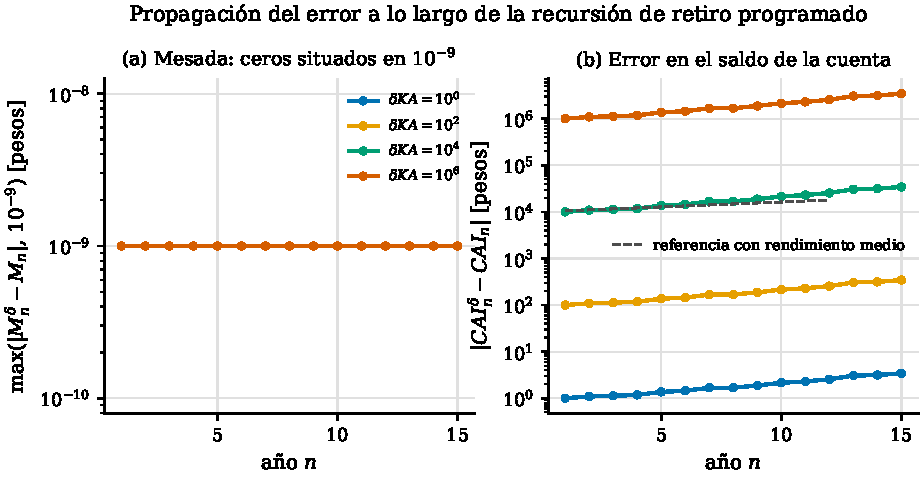
\includegraphics[width=\textwidth]{figuras/fig_propagacion_error_rp}
\caption[Propagación del error en retiro programado]{Experimento ilustrativo
con perturbaciones del capital inicial de $10^0$, $10^2$, $10^4$ y $10^6$
pesos, utilizando los mismos rendimientos en las trayectorias comparadas.
El panel (a) muestra las diferencias de mesada del escenario y el panel (b),
las diferencias de saldo. La línea discontinua es una referencia geométrica
construida con el rendimiento medio; no constituye una cota general cuando
los rendimientos varían. La absorción de perturbaciones depende del régimen
activo y de su dependencia de la mesada anterior (\cref{cor:regimenes}).}
\label{fig:propagacion}
\end{figure}

\begin{corollary}[Tolerancia admisible según el horizonte]
\label{cor:tolerancia-rp}
Bajo las hipótesis del \cref{thm:propagacion}, supóngase que el estado inicial
es el mismo en ambas trayectorias, $E_1=0$, y que
$\varepsilon_n^x\le\varepsilon_x$. Sea $e_1=(1,0)^{\mathsf T}$ y defínase
\[
 H_N^x=e_1^{\mathsf T}
 \sum_{j=1}^{N}\mathcal P_{N:j+1}
       \kappa\begin{pmatrix}G_j\\1\end{pmatrix}.
\]
Entonces $|\delta_{N+1}|\le H_N^x\varepsilon_x$. Si $H_N^x>0$, la condición
suficiente
\[
  \varepsilon_x\le\frac{\Delta}{H_N^x}
\]
garantiza un error del saldo final no mayor que $\Delta$.

Si la tolerancia anual se expresa en unidades de residuo,
$|\VP_n(U_n)-\widetilde C_n|\le\varepsilon_f$, y $U_n\in I_n$,
puede utilizarse $\varepsilon_n^x\le\varepsilon_f/m_n$. En ese caso basta
\[
 \varepsilon_f\le\frac{\Delta}{H_N^f},\qquad
 H_N^f=e_1^{\mathsf T}
 \sum_{j=1}^{N}\mathcal P_{N:j+1}
       \frac{\kappa}{m_j}\begin{pmatrix}G_j\\1\end{pmatrix},
\]
siempre que $H_N^f>0$.
\end{corollary}
\begin{proof}
Se toma la primera componente de la cota iterada del
\cref{thm:propagacion} y se utilizan, respectivamente,
$\varepsilon_j^x\le\varepsilon_x$ y
$\varepsilon_j^x\le\varepsilon_f/m_j$.
\end{proof}

El corolario distingue la tolerancia del residuo, medida en unidades de
capital, de la tolerancia de mesada. Su elección depende del horizonte,
las pendientes y la dependencia temporal de los ajustes. No se deduce un
factor universal de endurecimiento a partir del rendimiento medio y del
número de años solamente. La recomendación~R4 de la
\cref{sec:hallazgos-codigo} consiste en calibrar y verificar la tolerancia
para la configuración concreta de la proyección.

\section{El costo computacional del acoplamiento}

Una trayectoria de $N$ años requiere resolver hasta $N$ problemas de raíz.
Su costo es la suma de las llamadas efectivas al motor en esos años, incluyendo
la preparación de los datos y las derivadas. El promedio del banco de
cotizaciones de renta vitalicia no constituye por sí solo una medición del
costo de esta recursión: cambian las edades, las reservas financiables y
los ajustes activos. Las cifras de una trayectoria completa deben medirse
sobre esa trayectoria.

\begin{remark}[Arranque en caliente]
La mesada del año anterior puede utilizarse como punto inicial de la
valoración siguiente, expresada en la misma base monetaria. Si ese arranque
y la nueva raíz pertenecen al interior de un mismo tramo afín, el
apartado (i) del \cref{thm:terminacion-finita} garantiza que una propuesta de Newton con su pendiente
exacta alcanza la raíz; si se aplica una salvaguarda, debe verificarse además
que dicha propuesta se acepte. La proximidad de dos mesadas no demuestra
por sí sola esta condición, pues también cambia la función de valoración.
La ganancia del arranque en caliente requiere una medición específica y
no se le asigna un factor universal de aceleración.
\end{remark}

\section{Comparación entre las dos modalidades}

\begin{figure}[H]
\centering
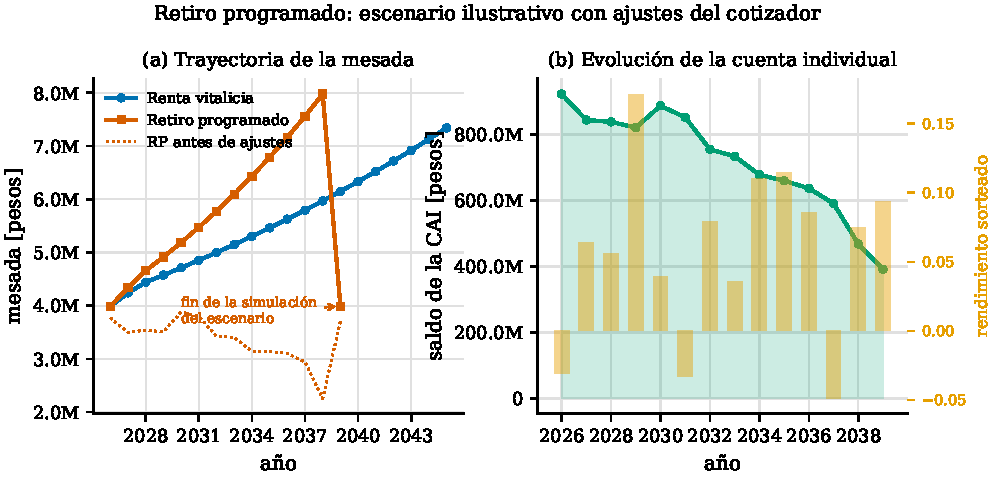
\includegraphics[width=\textwidth]{figuras/fig_rp_vs_rv}
\caption[Renta vitalicia frente a retiro programado]{Escenario ilustrativo
para una póliza. Panel (a): mesadas proyectadas bajo las hipótesis y reglas
del motor; la línea punteada muestra la mesada bruta de retiro programado
antes de los ajustes. El punto donde termina una serie indica la
interrupción de la simulación y no la extinción del derecho pensional.
Panel (b): evolución del saldo y rendimientos anuales sorteados. Una
trayectoria no establece una comparación general de los riesgos ni una
superioridad económica entre modalidades.}
\label{fig:rp-vs-rv}
\end{figure}

Las modalidades distribuyen de forma diferente los riesgos del pensionado y
de las entidades participantes. El escenario de la figura está condicionado
por los parámetros financieros, las reglas comerciales y los rendimientos
sorteados; en particular, el arranque puede estar fijado a la misma mesada
de renta vitalicia. Para comparar riesgos harían falta conjuntos de
trayectorias, hipótesis contrastadas y medidas de su distribución.

Desde el punto de vista numérico, las valoraciones anuales de retiro
programado pertenecen a la misma familia de máximos y recortes que la renta
vitalicia cuando sus coeficientes no dependen de la mesada buscada. No son
la misma función: los parámetros, las edades y los recargos pueden variar.
La estructura afín a trozos permite aprovechar derivadas laterales exactas
en cada problema, mientras que el acoplamiento temporal exige el control
del estado y de los errores locales establecido en este capítulo.
